%TODO:
% - fix example 2, 3 numbering: same example
% - references for algorithms
% - add speaker notes

% Copyright 2016 by Wang Kunzhen <wangkunzhen1993@gmail.com>.
%
% This is a latex template adapted from Till Tantau's Beamer template.
% It adds theme customizations for the convenience of users from the
% National University of Singapore. 
% 
% In principle, this file can be redistributed and/or modified under
% the terms of the GNU Public License, version 2.
%
% However, this file is supposed to be a template to be modified
% for your own needs. For this reason, if you use this file as a
% template and not specifically distribute it as part of a another
% package/program, I grant the extra permission to freely copy and
% modify this file as you see fit and even to delete this copyright
% notice. 

\documentclass[xcolor=dvipsnames]{beamer}
% \documentclass[notes]{beamer}       % print frame + notes
% \documentclass[notes=only]{beamer}   % only notes

\usepackage{tikz}
\usetikzlibrary{positioning}
\usepackage{algorithm}
\usepackage{algpseudocode}
\usepackage{algorithmicx}

\usepackage{mathtools}
\DeclarePairedDelimiter{\ceil}{\lceil}{\rceil}
\DeclarePairedDelimiter{\floor}{\lfloor}{\rfloor}
\DeclarePairedDelimiter{\vbar}{\vert}{\vert}
\DeclarePairedDelimiter{\vbarbar}{\Vert}{\Vert}
\DeclarePairedDelimiter{\parenLR}{\lparen}{\rparen}
\DeclarePairedDelimiter{\brackLR}{\lbrack}{\rbrack}
\DeclarePairedDelimiter{\braceLR}{\lbrace}{\rbrace}
\DeclarePairedDelimiter{\angleLR}{\langle}{\rangle}
\DeclareMathOperator*{\argmin}{arg\,min}
\DeclareMathOperator*{\argmax}{arg\,max}

\usepackage{amssymb}% http://ctan.org/pkg/amssymb
\usepackage{pifont}% http://ctan.org/pkg/pifont
\newcommand{\cmark}{\ding{51}}
\newcommand{\xmark}{\ding{55}}

\newcommand{\tup}[1]{\langle #1 \rangle}
\renewcommand{\cal}[1]{\mathcal{#1}}
\newcommand{\R}{\mathbb{R}}
\newcommand{\eps}{\varepsilon}
\newcommand{\Ch}{\mathit{Ch}}
\newcommand{\ch}{\mathit{ch}}
\newcommand{\Av}{\mathit{Av}}
\newcommand{\av}{\mathit{av}}
\newcommand{\CC}{\mathit{CC}}
\newcommand{\SCC}{\mathit{SCC}}
\newcommand{\core}{\mathit{Core}}
\newcommand{\I}{\mathit{I}}
\newcommand{\VI}{\mathit{VI}}
\newcommand{\AMI}{\mathit{AMI}}
\newcommand{\samples}{\omega}

\usepackage{biblatex}
\addbibresource{reference.bib}
\newcommand{\citenameyear}[1]{\citeauthor{#1}, (\citeyear{#1})}

% There are many different themes available for Beamer. A comprehensive
% list with examples is given here:
% http://deic.uab.es/~iblanes/beamer_gallery/index_by_theme.html
% You can uncomment the themes below if you would like to use a different
% one:
%\usetheme{AnnArbor}
%\usetheme{Antibes}
%\usetheme{Bergen}
% \usetheme{Berkeley}
%\usetheme{Berlin}
%\usetheme{Boadilla}
% \usetheme{boxes}
%\usetheme{CambridgeUS}
%\usetheme{Copenhagen}
%\usetheme{Darmstadt}
\usetheme{default}
%\usetheme{Frankfurt}
%\usetheme{Goettingen}
%\usetheme{Hannover}
% \usetheme{Ilmenau}
% \usetheme{JuanLesPins}
% \usetheme{Luebeck}
% \usetheme{Madrid}
% \usetheme{Malmoe}
%\usetheme{Marburg}
% \usetheme{Montpellier}
% \usetheme{PaloAlto}
% \usetheme{Pittsburgh}
% \usetheme{Rochester}
% \usetheme{Singapore}
% \usetheme{Szeged}
% \usetheme{Warsaw}

\usecolortheme{seagull}

\definecolor{nus-orange}{RGB}{239,124,0} 
\definecolor{nus-white}{RGB}{255,255,255}
\definecolor{nus-blue}{RGB}{0,61,124}
\definecolor{nus-black}{RGB}{0,0,0}

% Uncomment this section if you want the title background for each slide to be gradient like decaying from nus-orange to nus-white.
% \useoutertheme{shadow}
% \usepackage{tikz}
% \usetikzlibrary{shadings}
% \colorlet{titleleft}{nus-orange}
% \colorlet{titleright}{nus-orange!45!nus-white}
% \makeatletter
% \pgfdeclarehorizontalshading[titleleft,titleright]{beamer@frametitleshade}{\paperheight}{%
%   color(0pt)=(titleleft);
%   color(\paperwidth)=(titleright)}
% \makeatother
% End of gradient slide title effect.

% \setbeamercolor{section in head/foot}{bg=nus-blue, fg=nus-white}
% \setbeamercolor{subsection in head/foot}{bg=nus-blue, fg=nus-white}
% \setbeamercolor{frametitle}{bg=nus-orange, fg=nus-black}
% \setbeamercolor{title}{bg=nus-orange, fg=nus-white}
% \setbeamercolor{alerted text}{fg=nus-orange}
% \setbeamercolor{block title}{fg=nus-blue}
% \setbeamercolor{block body}{fg=nus-black}

\setbeamertemplate{theorems}[numbered]
\setbeamertemplate{propositions}[numbered]

\setbeamertemplate{caption}{\raggedright\insertcaption\par}
\setbeamerfont{caption}{size=\scriptsize}

\setbeamertemplate{bibliography item}{\insertbiblabel}

\setbeamertemplate{title page}[default][colsep=-4bp,rounded=true, shadow=true]

\title{Learning Cooperative Solution Concepts From Voting Behavior}

\subtitle{A Case Study on the Israeli Parliament}

\author{Lu Wei}

\institute[National University of Singapore] % (optional, but mostly needed)
{
  Department of Computer Science\\
  National University of Singapore
}

\titlegraphic{
   \includegraphics[width=2cm]{nus-logo}
}

\date{Jan 2020}

% Uncomment this, if you want the table of contents to pop up at
% the beginning of each subsection:
% \AtBeginSubsection[]
% {
%   \begin{frame}<beamer>{Outline}
%     \tableofcontents[currentsection,currentsubsection]
%   \end{frame}
% }

\begin{document}

\begin{frame}
  \titlepage
\end{frame}

\begin{frame}{Outline}
  \tableofcontents
\end{frame}

\section{Introduction}

\begin{frame}{Background}
  \begin{itemize}
    \item Coalition formation games:
      \note{A type of cooperative game where players, each with their own preferences, form groups (aka coalitions)}
    \begin{itemize}
      \item Mostly theoretical analysis
      \item Most models require full information on player preference
      \item Lack of large dataset with ground truth
    \end{itemize}
    \item Clustering \& community detection:
    \begin{itemize}
      \item Data-driven analysis
      \item Missing strategic behavior modelling
    \end{itemize}
  \end{itemize}
\end{frame}

\begin{frame}{Data}
  \begin{itemize}
    \item Israeli parliament (the Knesset) voting data
    \item Available since March 2017
    \item Contains 147 parliament members' votes on over 7500 bills in $\sim$ 4 years
    \item Ground truth clusters: political party affiliations
    \begin{itemize}
      \item 10 parties aligned along a left-right axis
      \item Ideological agreement among the government (right) and the opposition (left) parties respectively
    \end{itemize}
  \end{itemize}
\end{frame}

\begin{frame}{Probably Approximately Correct (PAC) Stability}
  \small
  Given $m$ observations of formed coalitions $S_1,\dots,S_m$ sampled i.i.d. from some distribution $\cal D$, and the cardinal valuations of players in $S_j$ $(v_i(S_j))_{i \in S}$
  \note{Assume that future coalitions will be sampled from the same distribution.}

  \textit{Local loss} given a coalition structure $\pi$ and a coalition $S \subseteq N$:
$$\lambda(\pi,S) = \begin{cases}1 & \mbox{if }\forall i \in S: v_i(S) > v_i(\pi(i))\\0&\mbox{otherwise.}\end{cases}$$
  \note{$\lambda(\pi,S)$ incurs a loss of 1 if $\pi$ was not able to hedge against the members of $S$ deviating from $\pi$.}
  The \textit{expected loss} of $\pi$ w.r.t. $\cal D$:
$$L_{\cal D}(\pi) = \Pr_{S \sim \cal D}\left[\lambda(\pi,S) =1\right]\label{eq:total-loss-D}$$

A \textit{PAC stabilizing} algorithm:
  \begin{itemize}
    \item input: a set of i.i.d. samples $S_1,\dots,S_m \sim \cal D^m$
    \item output: a coalition structure $\pi^*$  with the following guarantee:
    $\Pr_{(S_1,\dots,S_m)\sim \cal D^m}[L_{\cal D}(\pi^*) \ge \eps]< \delta \label{eq:pac-stable}$
    \item The number of samples needed $m$ grows linearly in the number of players, and polynomially in $\frac1\eps$ and $\log\frac1\delta$
  \end{itemize}


\end{frame}

\begin{frame}{Research Questions}
  \begin{itemize}
    \item Can we use hedonic games to model real-world collaborative activities?
    \item How well does the outcome compare to ground truth?
    \item How well does the outcome compare to that of canonical clustering and community detection models?
  \end{itemize}
\end{frame}

\section{Methodology}

\begin{frame}{Methodology}{Game Theoretic Models}
  \begin{itemize}
    \item Assumes hedonic preferences
      \note{Under Hedonic preferences, players only care about the makeup of the coalitions of which they are members; they are indifferent about the makeup of other coalitions}
    \begin{itemize}
      \item Top responsive
      \item Bottom responsive
      \item Boolean
    \end{itemize}
    \item<2-> Two approaches:
    \begin{itemize}
      \item Full-information models: construct complete preference profile, then derive core stable solution
      \item PAC models: learn a probably stable solution directly from partial preference relations
      \begin{itemize}
        \item<3-> Simulate i.i.d.: sampling with replacement 3/4 of all bills
        \item<3-> Repeat 50 times to check consistency of solution between runs
        \item<3-> Select the ``centroid'' to represent model output: partition with minimum sum of information distance from other 49 partitions
      \end{itemize}
    \end{itemize}
  \end{itemize}
\end{frame}

\begin{frame}{Methodology}{Comparisons}
  \begin{itemize}
    \item Comparison machine learning models:
    \begin{itemize}
      \item K-Means
      \item Stochastic Block Model
    \end{itemize}
    \item Comparing every hedonic \& ML model output partition to ground truth party affiliations
    \begin{itemize}
      \item Quantitatively: information theoretic measures
      \item Qualitatively: political analysis
    \end{itemize}
  \end{itemize}
\end{frame}

\begin{frame}{How different are two partitions, quantitatively?}{Objectives}
  We want a measure that\ldots
  \begin{itemize}
    \item has strong mathematical foundation: information theoretic measures
    \item is intuitive: satisfing metric property
    \begin{itemize}
      \item non-negativity
      \item symmetry
      \item triangle inequality
    \end{itemize}
  \end{itemize}
\end{frame}

\begin{frame}{How different are two partitions, quantitatively?}{Definitions}
  \begin{columns}
  \column{0.4\textwidth}
  \begin{figure}
    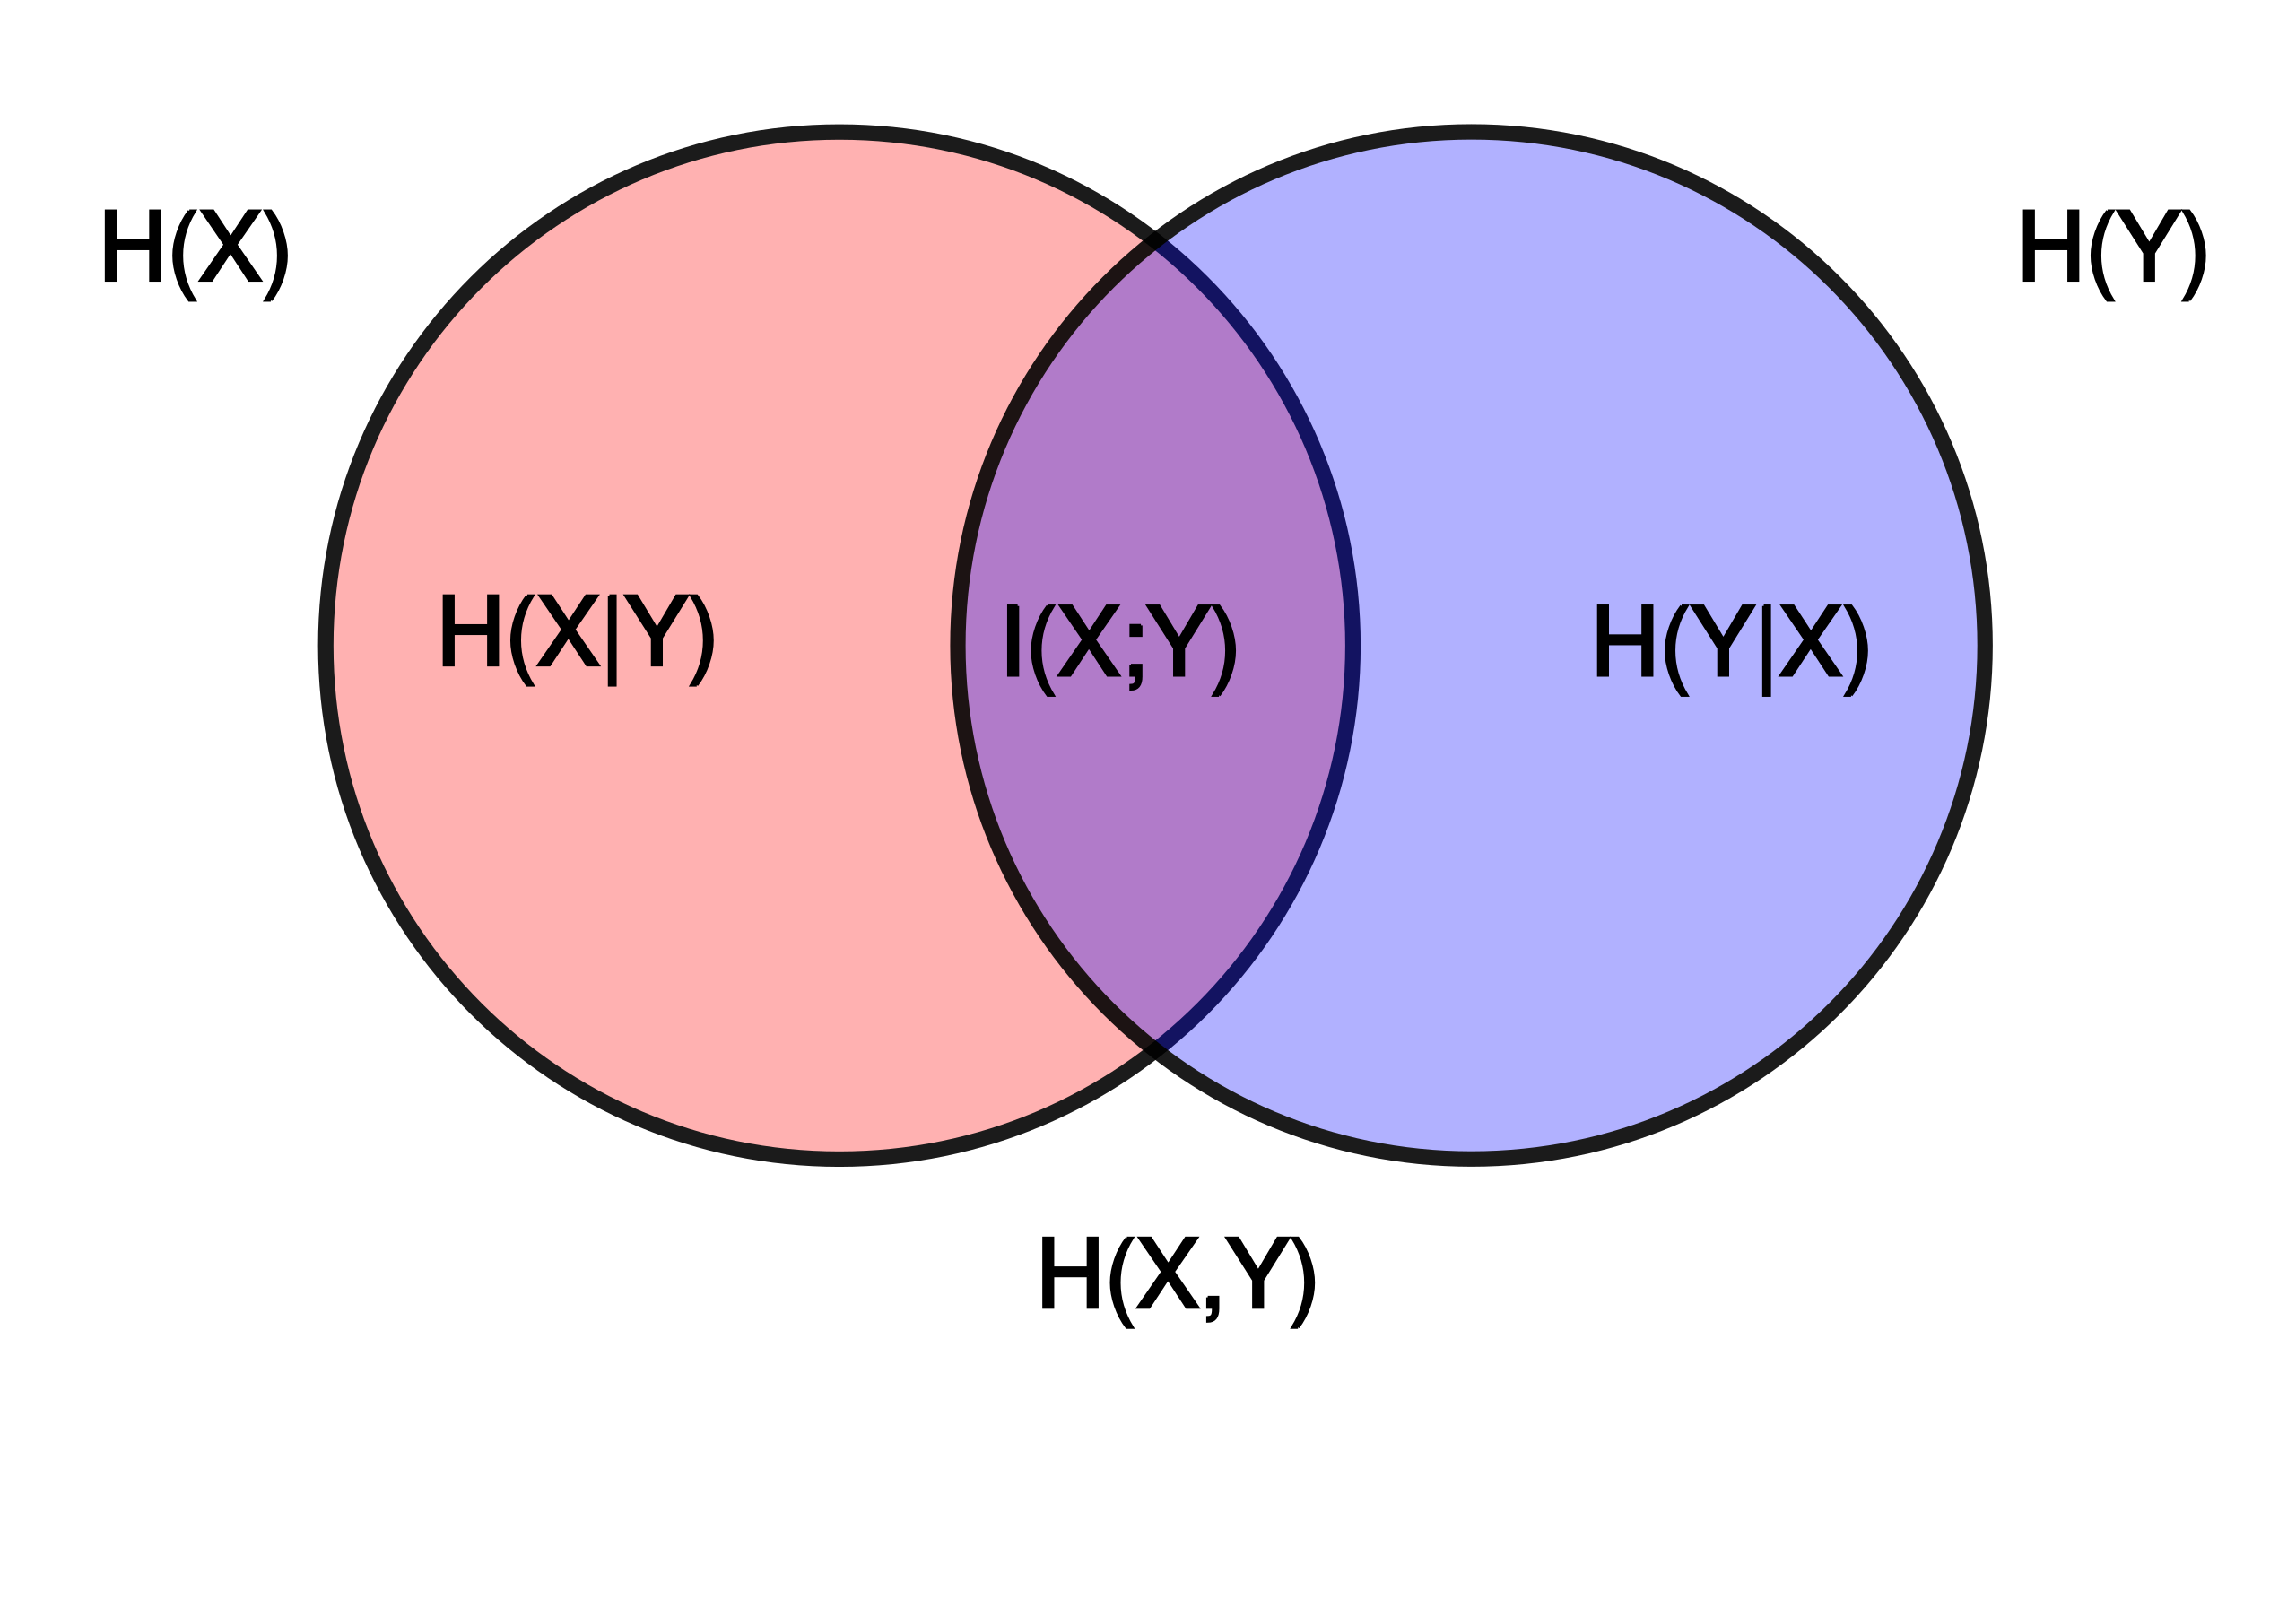
\includegraphics[width=\linewidth]{entropy-relation-diagram}
    \caption{Venn diagram showing additive and subtractive relationships various information measures associated with correlated variables X and Y}
  \end{figure}
  \column{0.6\textwidth}
  \begin{itemize}
    \item Entropy: $H(\pi) = - \sum^J_{j=1} \frac{|S_j|}{|N|} \log{\frac{|S_j|}{|N|}}$
    \item Conditional entropy: $H(\pi|\pi') = - \sum^J_{j=1} \sum^K_{k=1} \frac{|S_j \cap S'_k|}{|N|} \log{\frac{|S_j \cap S'_k|/|N|}{|S_k|/|N|}}$
    \item Mutual Information (MI): $\I(\pi, \pi') = H(\pi) - H(\pi|\pi')$
    \item Variation of Information (VI): $\VI(\pi, \pi') = H(\pi) + H(\pi') - 2\I(\pi, \pi')$, metric!
  \end{itemize}
  \end{columns}
\end{frame}

\begin{frame}{How different are two partitions, quantitatively?}{Baseline Values}
  \begin{columns}
  \column{0.5\textwidth}
  \begin{figure}
    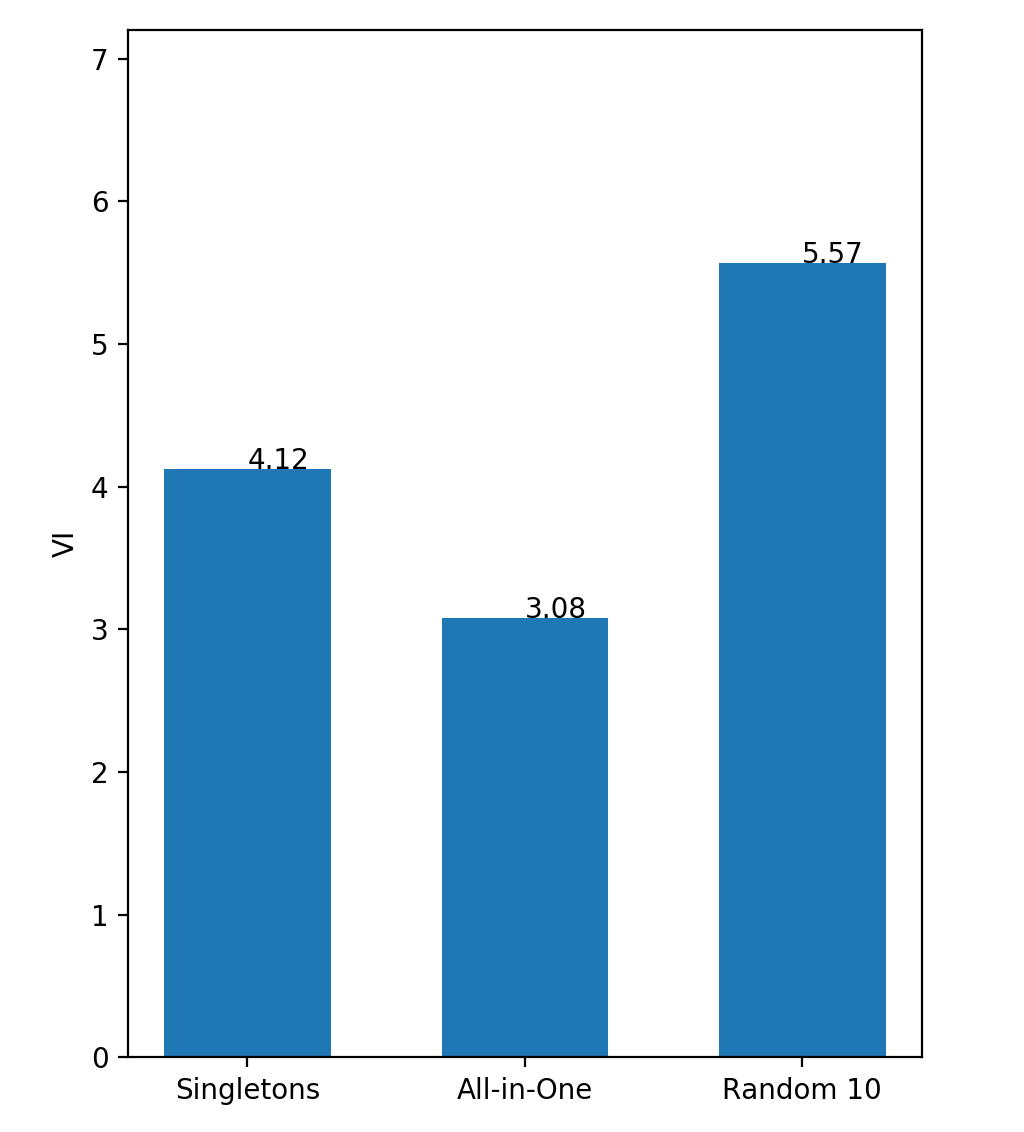
\includegraphics[width=\linewidth]{vi_baselines}
    \caption{The Knesset partition baseline VI values}
  \end{figure}
  \column{0.5\textwidth}
  \begin{figure}
    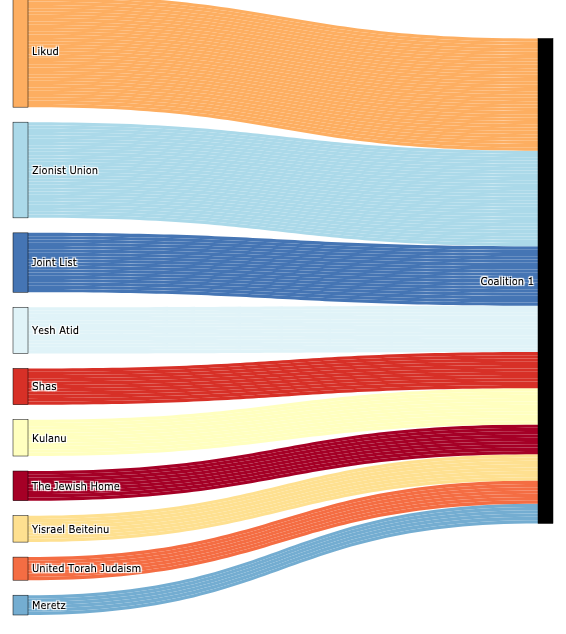
\includegraphics[width=\linewidth]{friends}
    \caption{All-in-One partition of the Knesset}
  \end{figure}
  \end{columns}
\end{frame}

\begin{frame}{How different are two partitions, quantitatively?}{Additional Measure: AMI}
  Adjusted Mutual Information (AMI):
  \[
    \AMI(\pi, \pi') = \frac{I(\pi, \pi') - E(I(\pi, \pi'))}{\max(H(\pi), H(\pi')) - E(I(\pi, \pi'))}
  \]
  \begin{itemize}
    \item Adjusted for chance
    \item Normalized: $\lbrack0, 1\rbrack$
    \item Not metric
  \end{itemize}

  Good for detecting ``bad'' (very different) partitions:
  \begin{table}[h]
  \centering
  \begin{tabular}{|c|c|}
  \hline
         & Ajusted Mutual Information \\ \hline
  Singletons & 3e-14 \\
  All-in-One & -5e-16 \\
  Randome 10 & 0.007 \\
  \hline
  \end{tabular}
  \caption{The Knesset partition baseline AMIs}
  \end{table}
\end{frame}


\section{Hedonic Game Stability Models}

\subsection{Top Responsive Games}
\begin{frame}{Top Responsive Games}{Definitions}
  Idea: for every player, the value of a coalition depends on the most preferred subset of players
  \begin{itemize}
    \item \textit{Choice sets}:
      $\Ch(i, S) = \{S' \subseteq S: (i \in S') \wedge (S' \succeq_i S'' \forall S'' \subseteq S)\}$\\
      When $|\Ch(i, S)| = 1$, the unique choice set is $\ch(i, S)$
      \note{A player i's most preferred set of coalitions}
    \item A \textit{top responsive} preference profile requires that for any player $i \in N$,
    and any coalition that may contain player $i$: $S, T \in \mathcal{N}_i$:
    \begin{enumerate}
      \item $|\Ch(i, S)| = 1$.
      \item if $\ch(i, S) \succ_i \ch(i, T)$ then $S \succ_i T$
      \item if $\ch(i, S) = \ch(i, T)$ and $S \subset T$ then $S \succ_i T$
    \end{enumerate}
    \note{In the context of our dataset, it captures the following idea: politicians care about whose votes they stand with; they want to vote with other politicians they like. If they can manage to pass a bill with fewer members involved, it is more efficient therefore more preferable.}
  \end{itemize}
\end{frame}

\begin{frame}{Top Responsive Games}{Example}
  \begin{example}
    \label{example:top_responsive_pref}
    \small
    Consider a game of three players with the following choice sets:

    $\ch(1, \{1, 2, 3\}) = \ch(1, \{1, 2\}) = \{1, 2\},
     \ch(1, \{1, 3\}) = \{1, 3\}, \ch(1, \{1\}) = \{1\}$

    $\ch(2, \{1, 2, 3\}) = \ch(2, \{2, 3\}) = \{2, 3\},
     \ch(2, \{1, 2\}) = \{1, 2\}, \ch(2, \{2\}) = \{2\}$

    $\ch(3, \{1, 2, 3\}) = \ch(3, \{1, 3\}) = \{1, 3\},
     \ch(3, \{1, 2\}) = \{1, 2\}, \ch(3, \{3\}) = \{3\}$
  \end{example}

  Then the resulting preference profile is top responsive:

  player 1: $\{1, 2\} \succ_1 \{1, 2, 3\} \succ_1 \{1, 3\} \succ_1  \{1\}$

  player 2: $\{2, 3\} \succ_2 \{1, 2, 3\} \succ_2 \{1, 2\} \succ_2  \{2\}$

  player 3: $\{1, 3\} \succ_3 \{1, 2, 3\} \succ_3 \{2, 3\} \succ_3  \{3\}$
\end{frame}

\begin{frame}{Top Responsive Games}{Core Finding Algorithms - Full Information}
  \begin{algorithm}[H]
    \small
    \caption{Top Covering Algorithm}
    \label{alg:top_covering}
    \textbf{Input:} A hedonic game satisfying top responsiveness.

    \begin{algorithmic}[1]
    \State $R^1 \leftarrow N$; $\pi \leftarrow \emptyset$.

    \For{$k=1$ to $|N|$}
      \State \label{top_cover:select} Select $S^k$
      \State \label{top_cover:remove} $\pi \leftarrow \pi \cup \lbrace S^k \rbrace$ and $R^{k+1} \leftarrow  R^k \setminus S^k$
      \If {$R^{k+1} = \emptyset$}
        \State \Return $\pi$
      \EndIf
    \EndFor

    \State \Return $\pi$
   \end{algorithmic}
  \end{algorithm}

  \small
  Let $C^1(i, S) = \ch(i, S)$ \note{for player $i \in S, S \subseteq N$}
  $C^{t + 1}(i, S) = \underset{j \in C^t(i, S)}{\bigcup} \ch(j, S)$ \note{where $t$ is a positive integer}

  The \textit{connected component} of $i$ with respect to $S$: $\CC(i, S) = C^{|N|}(i, S)$

  Step~\ref{top_cover:select}: select $i\in R^k$ such
  that $|\CC(i,R^k)| \leq |\CC(j,R^k)|$ for each $j\in R^k$;
  and $S^k\leftarrow \CC(i,R^k)$
\end{frame}

% dummy slide to take up algo numbering
\begin{frame}<presentation:0>[noframenumbering]{Top Responsive Games}{Core Finding Algorithms - PAC}
  \begin{algorithm}[H]
    \caption{Top Covering Algorithm - PAC}
    \textbf{Input:} A hedonic game satisfying top responsiveness.
    \begin{algorithmic}[1]
    \State \Return $\pi$
   \end{algorithmic}
  \end{algorithm}
\end{frame}

\begin{frame}{Top Responsive Games}{Core Finding Algorithms - PAC}
  \begin{columns}
  \column{0.5\textwidth}
  \begin{figure}
    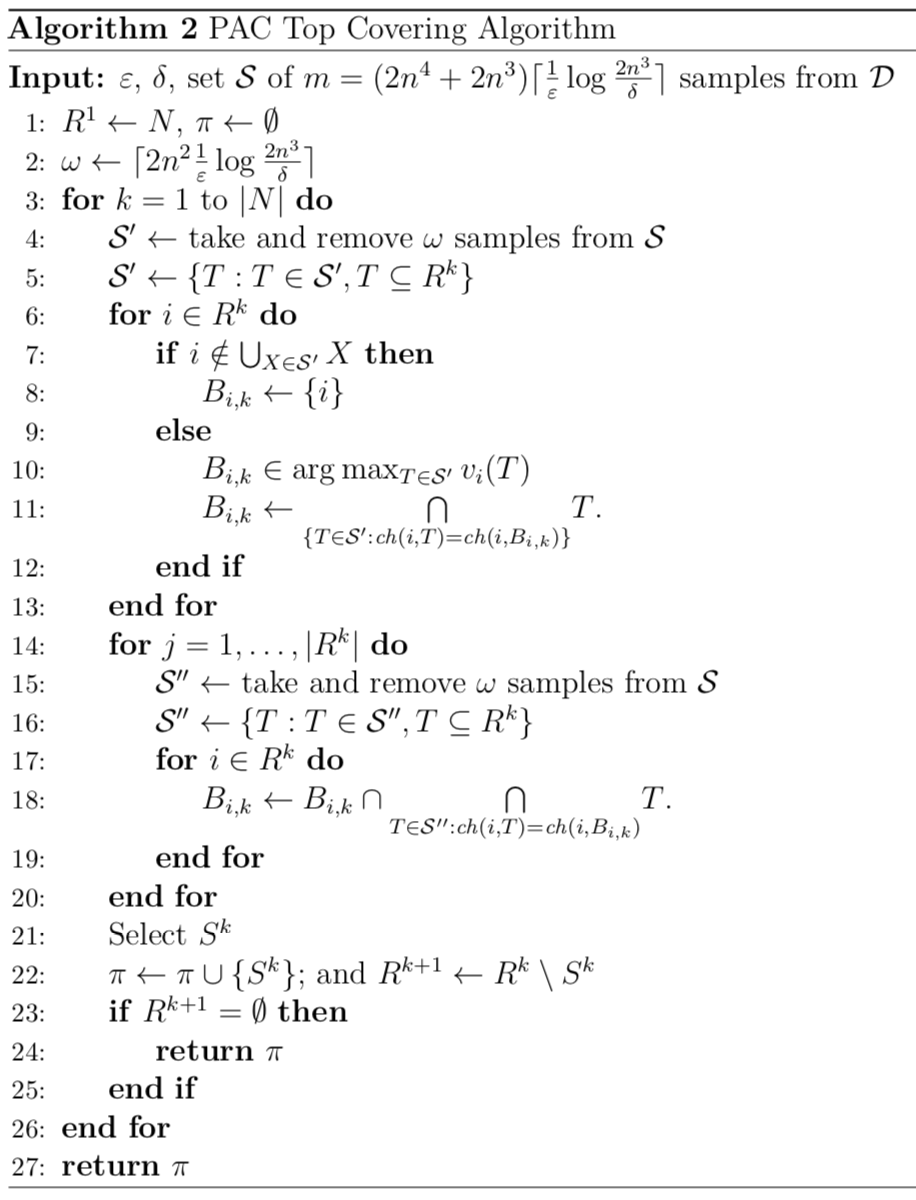
\includegraphics[width=\linewidth]{pac_top_cover}
  \end{figure}
  \column{0.5\textwidth}
  \begin{itemize}
    \scriptsize
    \item Steps 1-3, 21-27: the same structure as Algorithm~\ref{alg:top_covering}
    \item Steps 4-20: approximate player preferences from sample observations of coalitions formed
    \item Original \cite{ijcai2017-380} Step~21: select $i\in R^k$ such
                        that $|\CC(i,R^k)| \leq |\CC(j,R^k)|$ for each $j\in R^k$;
                        and $S^k\leftarrow \CC(i,R^k)$
    \item Improved Step~21: select the largest Strongly Connected Component (SCC)
                        in the graph induced by $R^k$ as vertices and directed edges $E$,
                        $(i, j) \in E$ if $j \in \ch(i, R^k)$ for all $j \in R^k$;
                        and $S^k\leftarrow \SCC(R^k)$
  \end{itemize}
  \end{columns}
\end{frame}

\begin{frame}{Top Responsive Games}{Imporoved Core Finding Algorithm - PAC}
  \begin{itemize}
    \item correctness proof
      \note whiteboarding, proof by picture
    \item running time improvements:
    \begin{itemize}
        \item each iteration: from finding smallest $\CC$'s $\mathcal{O}(|V|(|V| + |E|))$ to finding the largest $\SCC$'s $\mathcal{O}(|V| + |E|)$
        \item removing more players in the earlier iterations also reduces the amount of computation required for the later iterations
    \end{itemize}
  \end{itemize}
\end{frame}

\begin{frame}{Top Responsive Games - Handcrafted Value Function}

  Let $S_f$ be the set of members who voted ``for'' and $S_a$ be the set of members who voted ``against''.
  $S_p = S_f \cup S_a$.

  \begin{equation}
    v_i(S) =
    \begin{dcases}
        1 + \frac{1}{|S|} + \frac{|S_p|}{|N|},& \text{if $S$ is the winning majority}\\
        0,              & \text{otherwise}
    \end{dcases}
  \end{equation}

  \begin{itemize}
      \item<only@1> A winning coalition is always worth more than a losing coalition
        \note{winning: being successfully passing a bill or successfully blocking a bill}
      \item<only@1> $\frac{1}{|S|}$ reflects that a win is more valuable when achieved with fewer members
        \note{which is also conceptually consistent with top responsive game's preference for smaller coalitions}
      \item<only@1> The participation term $\frac{|S_p|}{|N|}$ gives a win more value when there are more effective votes for a given bill
      \item<only@1> Assign all unobserved coalition the value of zero
        \note{to ensure that the values for observed, winning coalitions are always
        greater than any unobserved coalition, because intuitively the existence of
        an observed coalition is evidence that every member in that coalition prefers
        to be a part of that coalition than some unobserved coalition}
      \item<only@2> Core stable partition: apply Algorithm~\ref{alg:top_covering} with partial reference profile as input
        \note{Although the original top covering algorithm expects the full preference
        profile as input, it would still terminate and produce a partition
        if the input is a partial preference profile.
        The produced partition ensures that any of the observed coalitions would
        have no incentive to deviate.}
      \item<only@2> PAC stable partition: apply improved Algorithm 2, sampling with replacement to make up for insufficient samples
  \end{itemize}
\end{frame}

\begin{frame}{Top Responsive Games - Appreciation of Friends}

  Let $G_i$ be player $i$'s set of friends, and $B_i$ the set of enemies.
  $G_i \cup B_i \cup i = N$ and $G_i \cap B_i = \emptyset$.
  A preference profile $P^f$ is based on \textit{appreciation of friends} if for all player $i \in N$,
  $S \succeq_i T$ if and only if
  \begin{enumerate}
    \item $|S \cap G_i| > |T \cap G_i|$ or
    \item $|S \cap G_i| = |T \cap G_i|$ and $|S \cap B_i| \leq |T \cap B_i|$
  \end{enumerate}

  \begin{itemize}
      \item<only@1> Friends: anyone whose votes agreed with the given player's more often than they disagreed
      \item<only@1> Agreed votes are only counted if the given player voted ``for'' or ``against''
      \item<only@1> Disagreed votes:
      \begin{enumerate}
        \item Narrow disagreement (general friends): the other player's vote is different from mine, and is either ``for'' or ``against''
        \item Broad disagreement (selective friends): the other player's vote is different from mine
      \end{enumerate}
      \note{Compared to narrow disagreement, broad disagreement leads to every player being
            more selective of friends; it may also break the symmetry of the friend relationship}
  \end{itemize}
\end{frame}

\begin{frame}{Top Responsive Games - Appreciation of Friends}{Examples}

\begin{example}
\label{example:votes_friends}
  \small
  Given 3 players and 3 bills, their votes are as follow:

  \begin{table}[ht]
  \centering
  \begin{tabular}{|c|c|c|c|}
  \hline
         & player 1  & player 2 & player 3 \\ \hline
  bill A & for       & for      & against \\
  bill B & abstained & for      & abstained \\
  bill C & abstained & against  & abstained \\
  \hline
  \end{tabular}
  \end{table}

\end{example}

\small
\alert{General friends} preference profile:

player 1: $\{1, 2\} \succ_1 \{1, 2, 3\} \succ_1 \{1\} \succ_1 \{1, 3\} $

player 2: $\{1, 2\} \succ_2 \{1, 2, 3\} \succ_2 \{2\} \succ_2 \{2, 3\}$

player 3: $\{3\} \succ_3 \{1, 3\} \sim \{2, 3\} \succ_3 \{1, 2, 3\}$

\alert{Selective friends} preference profile:

player 1: $\{1, 2\} \succ_1 \{1, 2, 3\} \succ_1 \{1\} \succ_1 \{1, 3\} $

player 2: $\{2\} \succ_2 \{1, 2\} \sim \{2, 3\} \succ_2 \{1, 2, 3\} $

player 3: $\{3\} \succ_3 \{1, 3\} \sim \{2, 3\} \succ_3 \{1, 2, 3\}$

\note{Under general friends, players 1 and 2 are friends because they agreed on bill A.
In comparison, under selective friends, from player 1's point of view, player 2
is still a friend due to bill A, while player 2 considers player 1 an enemy
because player 1 did not vote with her for bill B and C.}

\end{frame}


\subsection{Bottom Responsive Games}

\begin{frame}{Bottom Responsive Games}{Definitions}
  Idea: for every player, the value of a coalition depends on \alert{the absence of the least preferred} subset of players
  \begin{itemize}
    \item \textit{Avoid sets}:
      $\Av(i, S) = \{S' \subseteq S: (i \in S') \wedge (S' \preceq_i S'' \forall S'' \subseteq S)\}$
      \note{A player i's most disliked players}
    \item A \textit{bottom responsive} preference profile requires:

    \begin{enumerate}
      \item if for all $S' \in \Av(i, S)$ $T' \in \Av(i, T)$, $ S' \succ_i T'$
        then $S \succ_i T$
      \item if $\Av(i, S) \cap \Av(i, T) \neq \emptyset$ and $|S| \geq |T|$
        then $S \succeq_i T$
        \note{Different from top responsive game which breaks ``ties'' in favor of
        smaller coalitions, condition 2 of bottom responsive game breaks ``ties'' in
        favor of larger coalitions.}
    \end{enumerate}

    \note{In the context of our parliament voting dataset, by taking a bottom responsive
          model, we are implicitly assuming that parliament members care more about having
          no disagreements with people in the set of members who voted with them.}
  \end{itemize}
\end{frame}


\begin{frame}{Bottom Responsive Games - Aversion to Enemies}

  A preference profile $P^e$ is based on \textit{aversion to enemies} if for every
  player $i \in N$, $S \succeq_i T$ if and only if
  \begin{enumerate}
    \item $|S \cap B_i| < |T \cap B_i|$ or
    \item $|S \cap B_i| = |T \cap B_i|$ and $|S \cap G_i| \geq |T \cap G_i|$
  \end{enumerate}
  It is a proper subclass of bottom responsive games

  \begin{itemize}
      \item<only@1> Friends: anyone whose votes agreed with the given player's more often than they disagreed
      \item<only@1> Agreed votes are only counted if the given player voted ``for'' or ``against''
      \item<only@1> Disagreed votes:
      \begin{enumerate}
        \item Narrow disagreement (general friends/selective enemies): the other player's vote is different from mine, and is either ``for'' or ``against''
        \item Broad disagreement (selective friends/general enemies): the other player's vote is different from mine
      \end{enumerate}
  \end{itemize}
\end{frame}


\begin{frame}{Top Responsive Games - Aversion to Enemies}{Examples}

\begin{example} %same as example used in friends
  \small
  Given 3 players and 3 bills, their votes are as follow:

  \begin{table}[ht]
  \centering
  \begin{tabular}{|c|c|c|c|}
  \hline
         & player 1  & player 2 & player 3 \\ \hline
  bill A & for       & for      & against \\
  bill B & abstained & for      & abstained \\
  bill C & abstained & against  & abstained \\
  \hline
  \end{tabular}
  \end{table}

\end{example}

\small
\alert{General friends / selective enemies} preference profile:

player 1: $\{1, 2\} \succ_1 \{1\} \succ_1 \{1, 2, 3\} \succ_1 \{1, 3\} $

player 2: $\{1, 2\} \succ_2 \{2\} \succ_2 \{1, 2, 3\} \succ_2 \{2, 3\}$

player 3: $\{3\} \succ_3 \{1, 3\} \sim \{2, 3\} \succ_3 \{1, 2, 3\}$

\alert{Selective friends / general enemies} preference profile:

player 1: $\{1, 2\} \succ_1 \{1\} \succ_1 \{1, 2, 3\} \succ_1 \{1, 3\} $

player 2: $\{2\} \succ_2 \{1, 2\} \sim \{2, 3\} \succ_2 \{1, 2, 3\} $

player 3: $\{3\} \succ_3 \{1, 3\} \sim \{2, 3\} \succ_3 \{1, 2, 3\}$

\note{Notice that compared to the appreciation of friends model,
both players 1 and 2 now prefer their respective singleton coalition
over the grand coalition.
This illustrates that we can expect to observe smaller coalitions in partitions
generated from the enemy models compared to that from the friend models.}

\end{frame}


\begin{frame}{Bottom Responsive Games}{Core Finding Algorithms - Full Information}
  \begin{algorithm}[H]
    \caption{Bottom Responsive Game Core Finding Algorithm}
    \label{alg:bottom_responsive_core}
    \textbf{Input:} A bottom responsive game
    \begin{algorithmic}[1]

    \State $S \leftarrow N$; $\pi \leftarrow \emptyset$.
    \While {$S \neq \emptyset$}
      \State \label{bottom_responsive_core:select_begin} Set $\Gamma \leftarrow \{S\}$
      \State Set $\Phi \leftarrow \lbrace X \in \Gamma | \{i\} \in \Av(i, X) \text{ for each } i \in X \rbrace$
      \While {$\Phi = \emptyset$}
        \State $\Gamma \leftarrow \underset{X \in \Gamma}{\bigcup} \underset{i \in X}{\bigcup} \{ X \text{\textbackslash} \{j\} | j \in Y \text{ for some } Y \in \Av(i, X)\}$
        \State $\Phi \leftarrow \lbrace X \in \Gamma | \{i\} \in \Av(i, X) \text{ for each } i \in X \rbrace$
      \EndWhile
      \State \label{bottom_responsive_core:select_end} Select a coalition
        $X \in \Phi$
      \State \label{bottom_responsive_core:reduce} Set
        $\pi \leftarrow \pi \cup \lbrace X \rbrace$ and
        $S \leftarrow  S \setminus X$
    \EndWhile
    \State \Return $\pi$

    \end{algorithmic}
  \end{algorithm}
\end{frame}


\begin{frame}{Bottom Responsive Games}{Core Finding Algorithms - PAC}
  \begin{itemize}
    \item Same structure as Algorithm~\ref{alg:bottom_responsive_core}
    \item Approximate player preferences $\Av(i, X)$ from samples
    \begin{itemize}
      \item Find friends from each set of sample coalitions
      \item Take intersection of friend sets as ``true friends''
      \item Let each player's avoid set be players outside the ``true friends'' set
    \end{itemize}
  \end{itemize}
\end{frame}


\subsection{Boolean Hedonic Games}

\begin{frame}{Boolean Hedonic Games}
  Idea: a player either likes to be a member of a coalition or hates it
  \note{A player views any coalition she may belong to as either satisfactory or unsatisfactory.}
  \begin{itemize}
    \item A player is indifferent among all satisfactory coalitions, same for unsatisfactory coalitions
    \item Strictly prefers any satisfactory coalition over any unsatisfactory coalition
    \item Within each bill, ``for'' and ``against'' groups each forms a satisfactory coalition
    \item Assume unobserved coalitions as unsatisfactory
  \end{itemize}
\end{frame}


\begin{frame}{Boolean Hedonic Games}{Examples}
  \begin{example}
  \label{example:votes_boolean}
    Given a parliament with 3 players and 3 bills, their votes are as follow:

    \begin{table}[ht]
    \centering
    \begin{tabular}{|c|c|c|c|}
    \hline
           & player 1  & player 2 & player 3 \\ \hline
    bill A & for       & against  & for \\
    bill B & abstained & for      & for \\
    bill C & for       & against  & against \\
    \hline
    \end{tabular}
    \end{table}
  \end{example}

  \alert{Boolean} preference profile:

  player 1: $\{1, 3\} \sim \{1\} \succ_1 \{1, 2\} \sim \{1, 2, 3\}$

  player 2: $\{2\} \sim \{2, 3\} \succ_2 \{1, 2\} \sim \{1, 2, 3\}$

  player 3: $\{1, 3\} \sim \{2, 3\} \succ_3 \{3\} \sim \{1, 2, 3\}$

  \note{Observe that the preference profile formulated this way is symmetric ---
if a coalition is satisfactory for one player, it is also satisfactory for all
other players within it}
\end{frame}


\begin{frame}{Boolean Hedonic Games}{Core Finding Algorithms - Full Information}
  \begin{algorithm}[H]
    \scriptsize
    \caption{Boolean Hedonic Game Core Finding Algorithm}
    \label{alg:boolean_core}
    \textbf{Input:} A Boolean hedonic game
    \begin{algorithmic}[1]

    \State $N' \leftarrow N$; $\pi \leftarrow \emptyset$.
    \While {$N' \neq \emptyset$}
      \State \label{boolean_core:select} Find $S \subset N'$ where all players
        in $S$ find $S$ satisfactory, and the size of $S$ is the largest if there
        are multiple such coalitions.
      \State $\pi \leftarrow \pi \cup \lbrace S \rbrace$ and
        $N' \leftarrow  N' \setminus S$
    \EndWhile
    \State \Return $\pi$

    \end{algorithmic}
  \end{algorithm}

  \scriptsize
  \begin{itemize}
    \item Symmetry in preference profile implies the bill with the broadest support/disapproval also yields the largest coalition
    \item Symmetry further implies largest cross-party coalition will be part of the output partition
    \item Selecting any satisfactory coalition (not necessarily the largest) in Step~\ref{boolean_core:select} maintains core stability
    \item Our implementation: replace largest with median-sized coalition
  \end{itemize}
\end{frame}


\begin{frame}{Boolean Hedonic Games}{Core Finding Algorithms - PAC}
  \begin{itemize}
    \item Same as Algorithm~\ref{alg:boolean_core}
    \item Only difference: the input is satisfactory coalitions derived from sample bills
    \item The output is consistent with the observed samples, therefore PAC stable \cite{jha2019learning}
  \end{itemize}
\end{frame}

\section{Machine Learning Models}

\subsection{$k$-Means Clustering}
\begin{frame}{$k$-Means Clustering}
  $k$-means clustering\cite{Tan:2018:IDM:3208440} divides a given set of samples
  $x_1, \cdots, x_n$ into $k$ disjoint sets $C$, each described by the mean
  $\mu_j$ of the samples in the cluster;
  it produces a partition minimizing the \textit{within-cluster sum-of-squares} (WCSS):

  \[
      \sum_{i=1}^{n} \underset{\mu_j \in C}{\min}(||x_i - \mu_j||^2)
  \]

  \begin{itemize}
    \item General purpose
    \item Only need to find the best $k$
    \item Runs fast
    \item Assumes similar sized clusters
  \end{itemize}
\end{frame}

\begin{frame}{$k$-Means Clustering}{Model Construction}
  Distance between points
  \begin{itemize}
    \item Each politician correspond to a point
    \item Each bill acts as a feature
    \item A ``for'' vote takes value of 1, ``against'' -1, others 0
      \note{This simple vote value encoding captures the idea that ``for'' and ``against''
            votes are far from each other; anything else is neutral and is equidistant
            to ``for'' and ``against''.}
  \end{itemize}

  \begin{columns}
  \column{0.4\textwidth}
  Finding the best $k$
  \begin{itemize}
    \item Elbow method: $k=10$
    \item Average silhouette: $k=2$
  \end{itemize}

  \column{0.6\textwidth}
  \begin{figure}[H]
    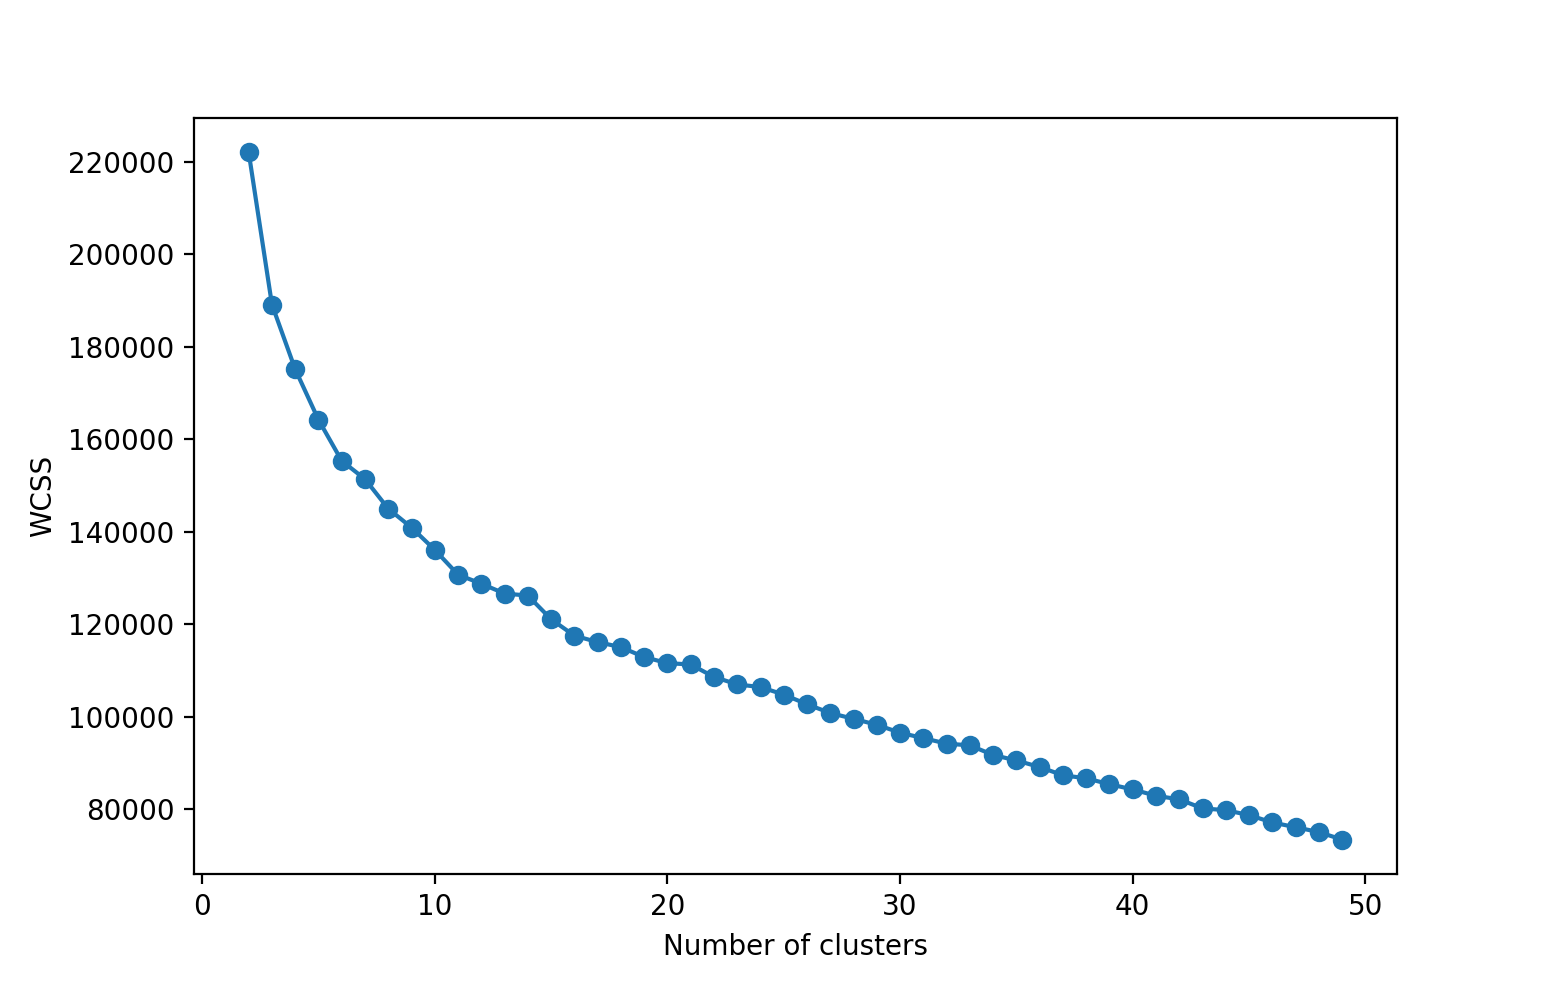
\includegraphics[width=\linewidth]{k_means_wcss}
    \label{Comparison:fig:k_means_wcss}
  \end{figure}
  \end{columns}
\end{frame}


\subsection{Stochastic Block Model}

\begin{frame}{Stochastic Block Model}
  \begin{itemize}
    \item A benchmark model in community detection
    \item Models dataset as a graph: parliament members as nodes, same/different votes as edge weights
    \item Assumes nodes in the same block shares same probability of being connected to other nodes
    \item Using Bayesian inference to find a partition that maximizes the likelihood of the observed network
  \end{itemize}
\end{frame}

\begin{frame}{Stochastic Block Model}{Modeling Edge Weights}
  \scriptsize
  \begin{columns}
  \column{0.5\textwidth}
  \begin{itemize}
    \item Positive edge weight: the number of times a pair of politicians voted together, either ``for'' or ``against'' a bill.
    \item Modeled as a geometric distribution
  \end{itemize}
  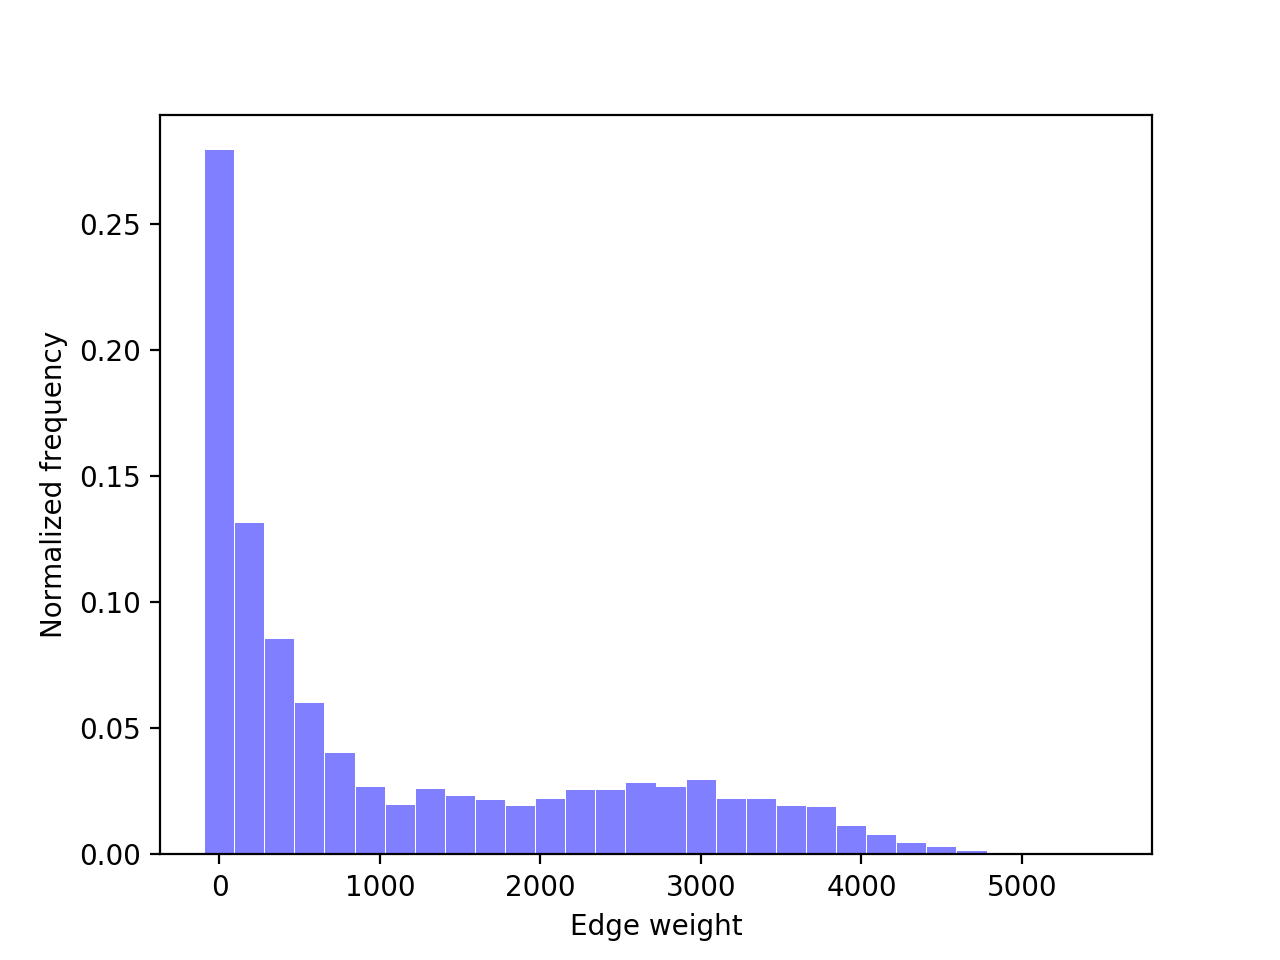
\includegraphics[width=\linewidth]{sbm_edge_weight_hist}

  \column{0.5\textwidth}
  \begin{itemize}
    \item Possibly negative edge weight: the difference between the number of times their votes agree and the number of times their votes disagree
    \item Modeled as a normal distribution
  \end{itemize}
  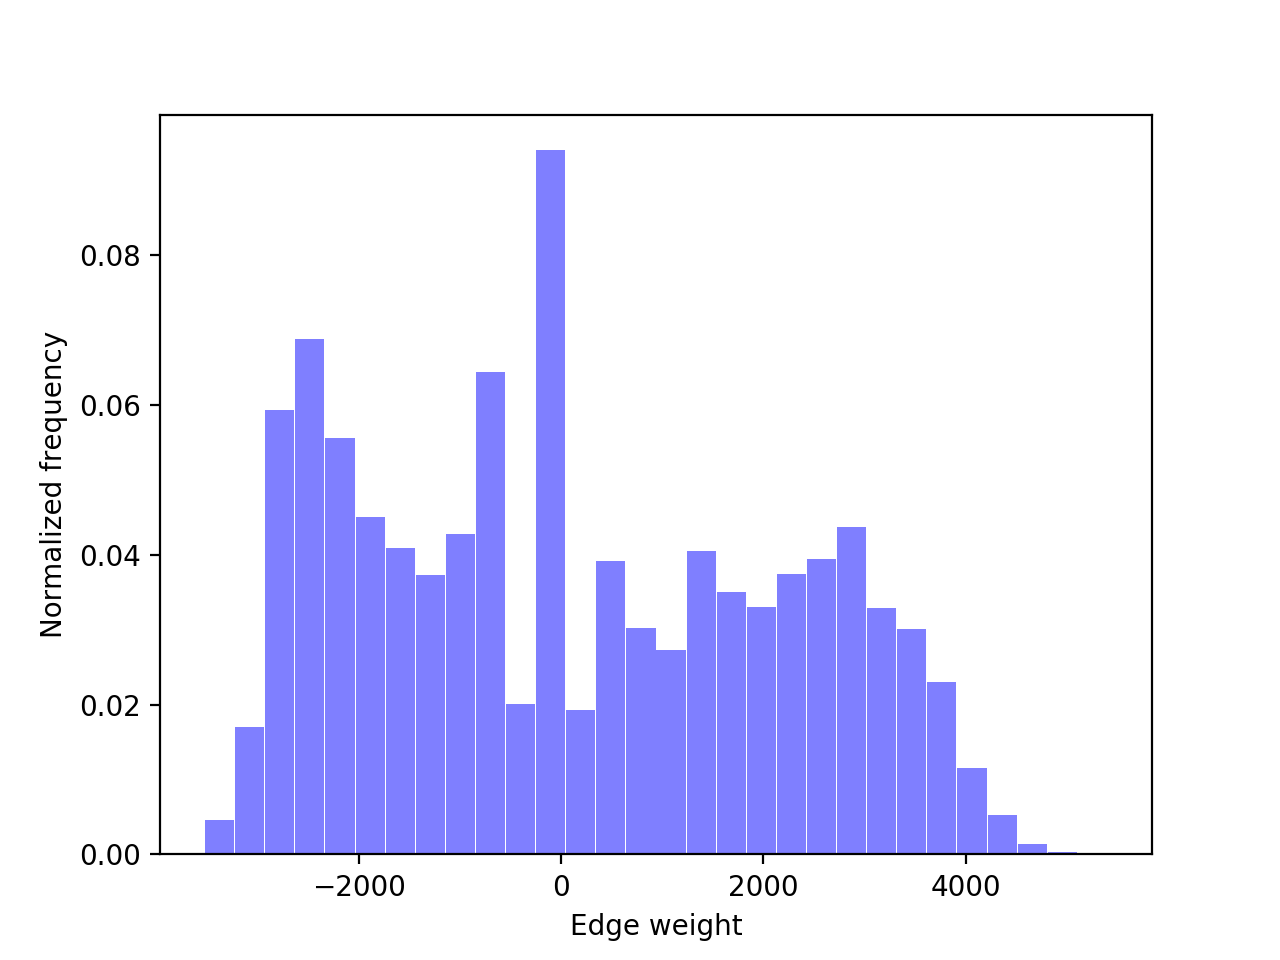
\includegraphics[width=\linewidth]{sbm_edge_weight_neg_hist}
  \end{columns}
\end{frame}

\section{Results \& Discussion}

\begin{frame}{Variability among PAC Partitions}
  \small
  \begin{table}[H]
  \centering
  \begin{tabular}{|c|c|c|}
  \hline
    Model & Partition Size Mean (SD) & CV \\ \hline
  Value Function & 87 (0) & 0 \\
  General Friends & 13 (1.29) & 0.10  \\
  Selective Friends & 20 (1.83) & 0.09  \\
  Selective Enemies & 10 (0) & 0 \\
  General Enemies & 34 (0.84) & 0.02 \\
  Boolean & 85 (16.92) & 0.2  \\
  \hline
  \end{tabular}
  \caption{PAC model partition size statistics across 50 runs per model}
  \label{Analysis:table:pac_num_coalitions}
  \end{table}

  \begin{table}[H]
  \centering
  \begin{tabular}{|c|c|c|}
  \hline
    Model & Pairwise AMI Mean (Min) & CV \\ \hline
  Value Function & 1 (1) & 0 \\
  General Friends & 0.78 (0.6) & 0.09  \\
  Selective Friends & 0.84 (0.66) & 0.08  \\
  Selective Enemies & 0.99 (0.97) & 0.01 \\
  General Enemies & 0.97 (0.93) & 0.01 \\
  Boolean & 0.18 (-0.06) & 0.86  \\
  \hline
  \end{tabular}
  \caption{PAC Model Partition Pairwise AMI Statistics over 50 Runs per Model}
  \label{Analysis:table:pac_pairwise_amis}
  \end{table}

\end{frame}


\begin{frame}{Quantitative Analysis}{AMI}
  \begin{figure}[H]
    \centering
    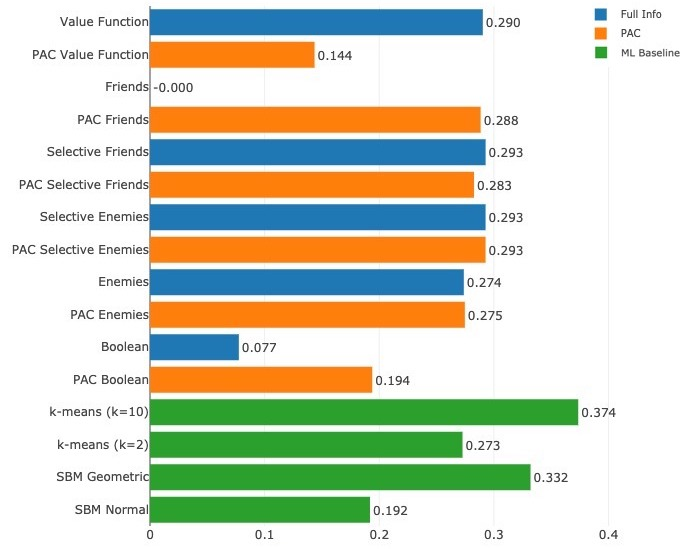
\includegraphics[width=0.7\linewidth]{ami}
    \caption{AMI between model partition and party affiliations}
    \label{Analysis:fig:ami}
  \end{figure}
\end{frame}

\begin{frame}{Quantitative Analysis}{Friends Models - Full Information}
  \small
  \begin{columns}
  \column{0.4\textwidth}
  \begin{figure}
    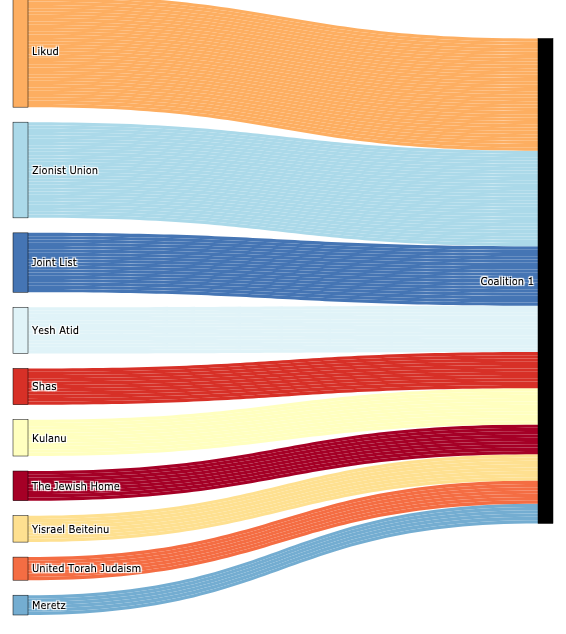
\includegraphics[width=\linewidth]{friends}
    \caption{General friends model output}
  \end{figure}
  \column{0.6\textwidth}
  Full-information models
  \begin{itemize}
    \item $\AMI_{\text{friends}} = 0$
    \item $\AMI_{\text{selective friends}} = 0.293$
    \item More friendly $\rightarrow$ more likely to have grand coalition as final partition
    \item Major drawback of the full-information friends models: sensitive to the definition of ``friends''
  \end{itemize}
  \end{columns}
\end{frame}


\begin{frame}{Quantitative Analysis}{Friends Models - PAC}
  \small
  \begin{columns}
  \column{0.4\textwidth}
  \begin{figure}
    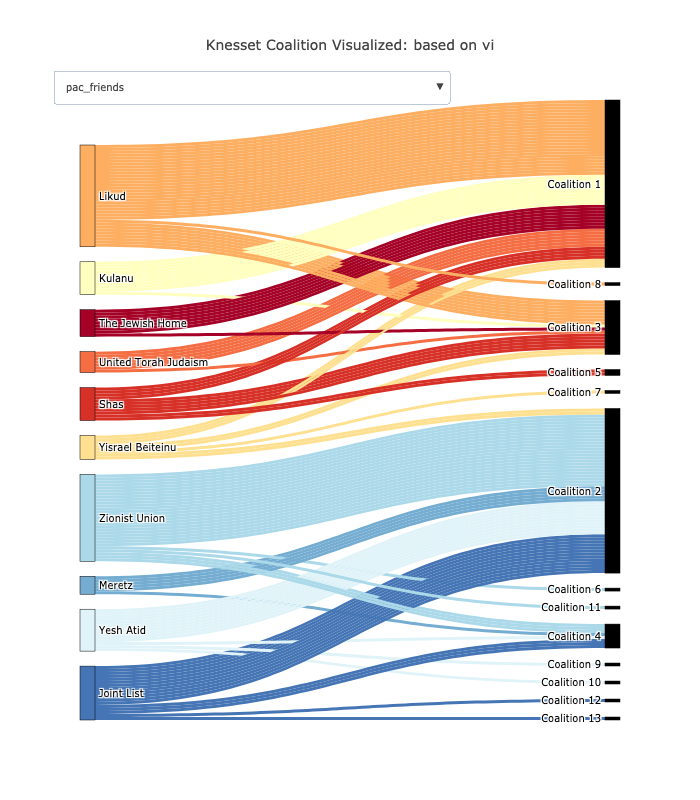
\includegraphics[width=\linewidth]{friends_pac}
    \caption{PAC general friends model output}
  \end{figure}
  \column{0.6\textwidth}
  PAC models
  \begin{itemize}
    \item $\AMI_{\text{PAC friends}} = 0.288$
    \item $\AMI_{\text{PAC selective friends}} = 0.283$
    \item PAC models dampen their sensitivity to the definition of friends through sampling
  \end{itemize}
  \end{columns}
\end{frame}


\begin{frame}{Quantitative Analysis}{Boolean Models}
  \small
  \begin{columns}
  \column{0.4\textwidth}
  \begin{figure}
    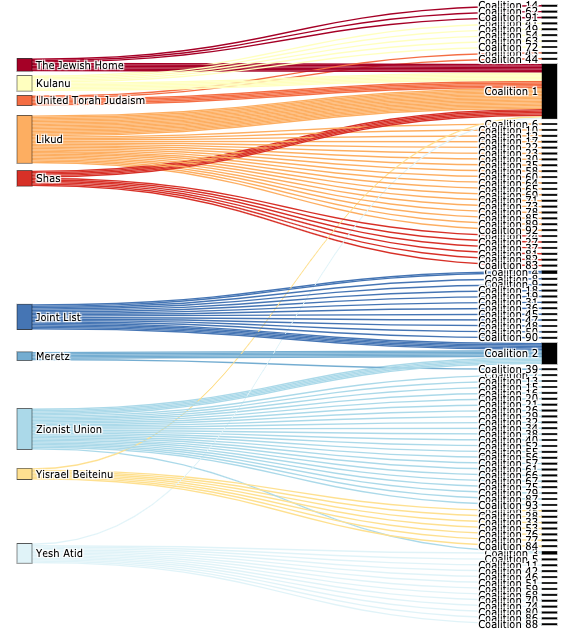
\includegraphics[width=\linewidth]{boolean}
    \caption{Boolean model output}
  \end{figure}
  \column{0.6\textwidth}
  Full-info model
  \begin{itemize}
    \item $\AMI_{\text{Boolean}} = 0.077$
    \item Too many ``stranded'' singleton coalitions
      \note{This is a result of a combination of the preference model and the core finding
algorithm for Boolean hedonic games:
Once a satisfying coalition $S$ is formed, we remove any other approved
coalitions that intersect with $S$; this effectively removes many satisfactory
coalitions for the remaining players.
If many players are left without satisfactory coalitions, they will be
``stranded'' in singleton coalitions, as observed.}
  \end{itemize}
  PAC model
  \begin{itemize}
    \item $\AMI_{\text{PAC Boolean}} = 0.194$
    \item Slightly better performance
    \item But of limited representativeness due to high variability
  \end{itemize}
  \end{columns}
\end{frame}


\begin{frame}{Quantitative Analysis}{Handcrafted Value Function Models}
  \small
  \begin{columns}
  \column{0.5\textwidth}
  \begin{figure}
    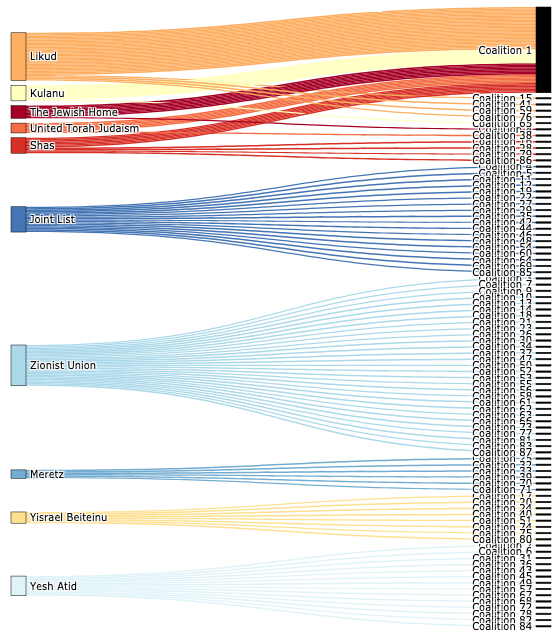
\includegraphics[width=\linewidth]{value_function_pac}
    \caption{PAC value function model output}
  \end{figure}
  \column{0.5\textwidth}
  \begin{figure}
    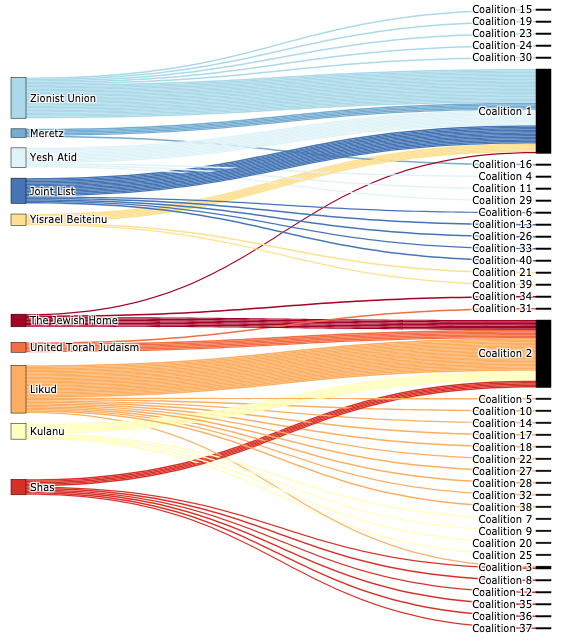
\includegraphics[width=\linewidth]{value_function}
    \caption{Value function model output}
  \end{figure}
  \end{columns}
\end{frame}

\begin{frame}{Quantitative Analysis}{Handcrafted Value Function Models}
  Full-info model
  \begin{itemize}
    \item $\AMI_{\text{Value Fuction}} = 0.290$
    \item Identified a government coalition and an opposition coalition
    \item Precense of Yisrael Beiteinu members in coalition 1 (opposition parties) not in line with reality
  \end{itemize}
  PAC model
  \begin{itemize}
    \item $\AMI_{\text{PAC Value Fuction}} = 0.144$
    \item Worst performing PAC model
    \item Many singleton coalitions
    \item Identified a government coalition
    \item Missing opposition coalition due to sampling more likely picking government majority bills --- limitation of value function formulation
      \note{One possible reason why we observe the opposition coalition dissolve while the
government coalition remains in the PAC version of the model is that the
government party members has a dominating advantage in the Knesset --- since our
value function (Function~\ref{eq:value_function}) values a winning majority over
a losing coalition, the parties forming the government more frequently pass
or oppose bills successfully than the opposition, therefore they are more
likely getting picked by the PAC sampling process.}
  \end{itemize}
\end{frame}


\begin{frame}{Quantitative Analysis}{SMB - Normal Edge Weights}
  \small
  \begin{columns}
  \column{0.5\textwidth}
  \begin{figure}
    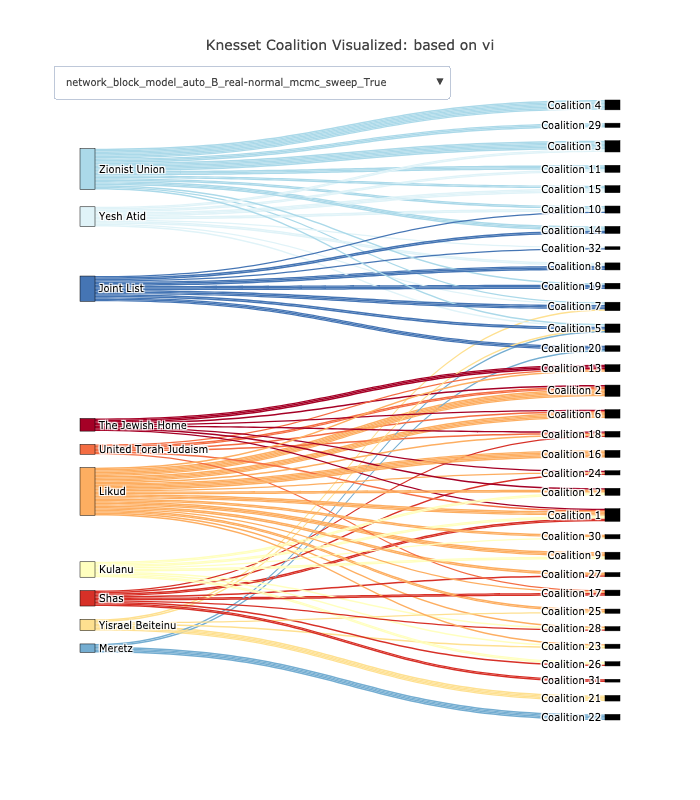
\includegraphics[width=\linewidth]{sbm_norm}
    \caption{SBM normal model output}
  \end{figure}
  \column{0.5\textwidth}
  \begin{itemize}
    \item $\AMI_{\text{SBM normal}} = 0.192$
    \item Many small coalitions
    \item Left-wing/right-wing grouping observed, but fails to distinguish the government from the opposition
  \end{itemize}
  \end{columns}
\end{frame}


\begin{frame}{Quantitative Analysis}{Model Selection}
  \small
  \begin{columns}
  \column{0.5\textwidth}
  \begin{figure}
    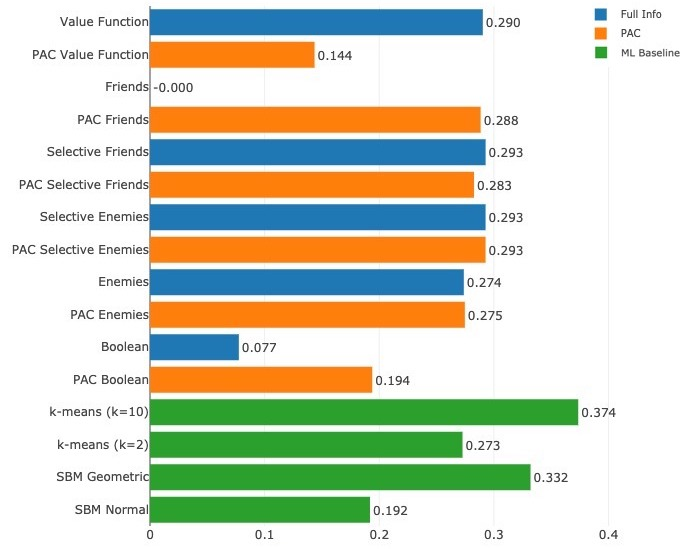
\includegraphics[width=\linewidth]{ami}
    \caption{AMI: higher means closer to ground truth}
  \end{figure}
  \column{0.5\textwidth}
  \begin{figure}
    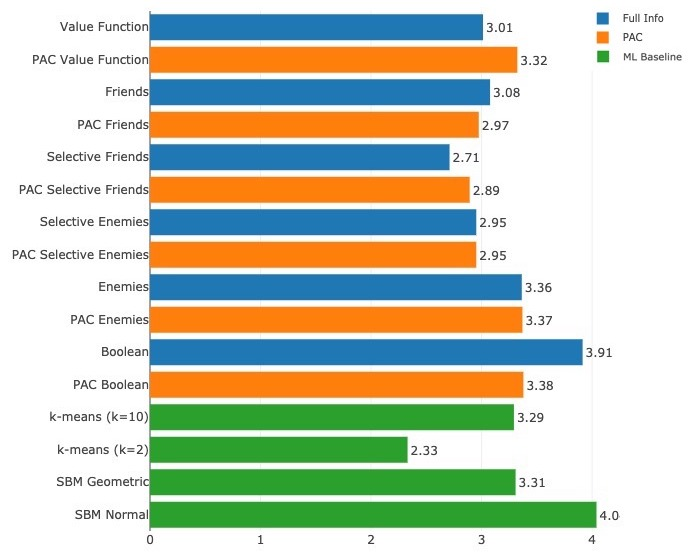
\includegraphics[width=\linewidth]{vi}
    \caption{VI: lower means closer to ground truth}
  \end{figure}
  \end{columns}
\end{frame}


\begin{frame}{Qualitative Analysis}{Selected Models}
  PAC Models
  \begin{itemize}
    \item Selective Friends
    \item Selective Enemies
    \item Boolean
  \end{itemize}
  Comparison ML Models
  \begin{itemize}
    \item 2-group $k$-means
    \item 10-group $k$-means
    \item SBM Geometric
  \end{itemize}
\end{frame}


\begin{frame}{Qualitative Analysis}
  Criteria
  \begin{itemize}
    \item Coherence: separate coalition and opposition parties cleanly? (no mixed coalitions)
    \item Overal Structure: able to distinguish between the main government and opposition groups?
    \item Party Sub-groups: able to identify subgroups within parties?
  \end{itemize}

  \begin{table}[H]
  \centering
  \begin{tabular}{|c|c|c|c|}
  \hline
    Model & Coherence & Structure & Sub-group \\ \hline
  PAC Selective Friends & \cmark & \cmark & \xmark \\
  PAC Selective Enemies & \cmark & \cmark & \xmark \\
  PAC Boolean & \cmark & \cmark & \xmark  \\
  2-group $k$-means & \xmark & \cmark & \xmark \\
  10-group $k$-means & \xmark & \xmark & \xmark \\
  SBM Geometric & \xmark & \xmark & \xmark \\
  \hline
  \end{tabular}
  \end{table}

\end{frame}

\section{Conclusion}

\begin{frame}{Conclusion}
  Summary
  \begin{itemize}
    \item ML methods: do not consider players' preferences and strategic behavior
    \item Game theoretic research: mostly theoretical or prescriptive with simulated data
    \item This thesis: a ``descriptive'' study of hedonic game theoretical models using real-world data of scale, and with ground truth
    \begin{itemize}
      \item PAC models are able to recover overall structure \& more coherent than ML models
      \item PAC approach result is more robust than full-info approach
        \note{By comparing the PAC and full-information settings for the friends models, we
observe that through sampling, PAC models produce partition results that are
more robust --- sampling helps ``dampen'' the model's sensitivity to the
definition of friends.}
    \end{itemize}
  \end{itemize}

  Future Research
  \begin{itemize}
  \item Apply PAC models on other parliaments, e.g. Dutch, Brazilian, US congress
  \item Apply other hedonic uncertainty models, e.g. Baysian core, on the Knesset dataset
  \end{itemize}
\end{frame}


% Placing a * after \section means it will not show in the outline or table of contents.
\section*{Bibliography}
\begin{frame}[allowframebreaks]{Bibliography}
  \printbibliography
\end{frame}

\end{document}
